\chapter{Ogólny opis systemu}
\label{cha:wprowadzenie}


\section{Cel (przeznaczenie) systemu}
\label{sec:celePracy}

Celem systemu automatyczny parking jest umożliwienie komputerowej obsługi pobierania opłat za~pozostawienie pojazdu na parkingu na określony czas.

\section{Udziałowcy i użytkownicy}

\begin{list}{$\bullet$}{}
\item Właściciel
\item Klient
\item Operator
\end{list}

\section{Podstawowe cele udziałowców i użytkowników}

\begin{table}[H]
	\begin{tabular}{|l|l|l|} \hline
	\textbf{Udziałowcy}	& \textbf{Cel} & \textbf{Priorytet} \\ \hline% \bottomrule
	Klient	& Wjechanie na parking & Wysoki \\
	Klient	& Opuszczenie parkingu & Wysoki \\
	%Klient	& Wpisanie numeru rejestracyjnego & Wysoki \\
	%Klient	& Potwierdzenie zdjęcia & Wysoki \\
	%Klient	& Anulowanie wpisanego numeru rejestracyjnego & Wysoki \\
	%Klient	& Uiszczenie opłaty & Wysoki \\
	Operator& Przeglądanie zdjęć & Wysoki \\
	Właściciel& Wyświetlenie statystyk & Średni \\ \hline
	\end{tabular}
\end{table}

% TODO:
% "Porównać sposób ich realizacji w aktualnym systemie (np.: manualnym)
% i systemie proponowanym"

\section{Granice systemu}

\begin{figure}[H]
	\centering
	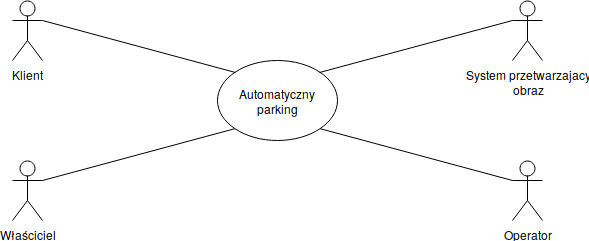
\includegraphics[width=90mm]{diagramy/graniceSystemu.jpg}
	\caption{Granice systemu automatyczny parking \label{overflow}}
\end{figure}

\section{Lista funkcji systemu}

\begin{figure}[H]
	\centering
	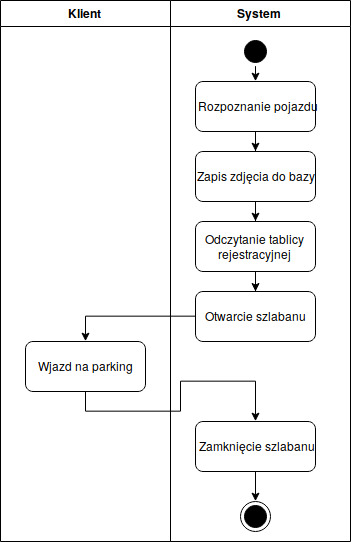
\includegraphics[width=90mm]{diagramy/DiagCzynWjazd.jpg}
	\caption{Diagram czynności: Klient wjeżdża na parking \label{overflow}}
\end{figure}

\begin{figure}[H]
	\centering
	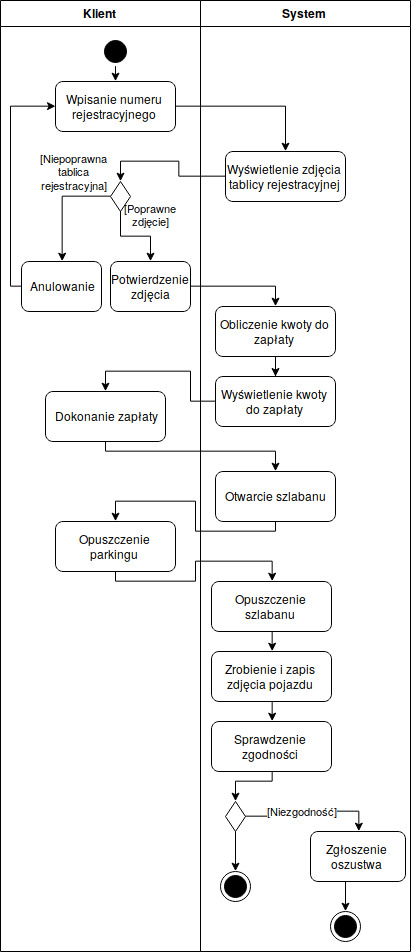
\includegraphics[width=90mm]{diagramy/DiagCzynWyjazd.jpg}
	\caption{Diagram czynności: Klient opuszcza parking \label{overflow}}
\end{figure}

% TODO:
% jeszcze diagram czynności dla Wyświetlania statystyk (Operator, System) 
% oraz Przeglądania zdjęć (Właściciel, System)


